\documentclass{article}

% if you need to pass options to natbib, use, e.g.:
%     \PassOptionsToPackage{numbers, compress}{natbib}
% before loading neurips_2020

% ready for submission
% \usepackage{neurips_2020}

% to compile a preprint version, e.g., for submission to arXiv, add add the
% [preprint] option:
%     \usepackage[preprint]{neurips_2020}

% to compile a camera-ready version, add the [final] option, e.g.:
%     \usepackage[final]{neurips_2020}

% to avoid loading the natbib package, add option nonatbib:
\usepackage[nonatbib]{neurips_2020}

\usepackage[utf8]{inputenc} % allow utf-8 input
\usepackage[T1]{fontenc}    % use 8-bit T1 fonts
\usepackage{hyperref}       % hyperlinks
\usepackage{url}            % simple URL typesetting
\usepackage{booktabs}       % professional-quality tables
\usepackage{amsfonts}       % blackboard math symbols
\usepackage{nicefrac}       % compact symbols for 1/2, etc.
\usepackage{microtype}      % microtypography
\usepackage{graphicx}
\usepackage{caption}
\usepackage{subcaption}


\title{Motivating Exploration in Reinforcement Learning}

% The \author macro works with any number of authors. There are two commands
% used to separate the names and addresses of multiple authors: \And and \AND.
%
% Using \And between authors leaves it to LaTeX to determine where to break the
% lines. Using \AND forces a line break at that point. So, if LaTeX puts 3 of 4
% authors names on the first line, and the last on the second line, try using
% \AND instead of \And before the third author name.

\author{
  Bob Wei\\
  Department of Computer Science\\
  University of Waterloo\\
  \texttt{q25wei@uwaterloo.ca} \\
  % examples of more authors
  \And
  Akshay Patel \\
  Department of Computer Science\\
  University of Waterloo\\
  \texttt{akshay.patel@uwaterloo.ca} \\
  \AND
  Samir Alazzam \\
  Department of Computer Science\\
  University of Waterloo\\
  \texttt{salazzam@uwaterloo.ca} \\
}

\begin{document}

\maketitle

\begin{abstract}
Self-motivation and curiosity come second nature to humans, both of which are crucial in quickly adapting to new environments and achieving distant goals. Using this as inspiration for artificial agents trained with reinforcement learning, we present an analysis of different techniques used by the current state-of-the-art to encourage exploration in varying environments. Specifically, we focus on formulations for entropy and curiosity, which promote exploration via randomness and state-based novelty respectively. We show that such methods are invariant to task/environment specifics, such as the reward density, and we also demonstrate that curious learners train faster based on extrinsic rewards and game visualizations.
\end{abstract}

\section{Introduction}

Exploration is something that comes naturally to humans, almost as if there exists an innate sense of curiosity, craving to experience something new, something yet to be seen. Jean Piaget, a Swiss developmental psychologist, asserted that it is in human nature to be curious, inquisitive, and interested in novelty as they develop and acquire knowledge about their environment \cite{piaget}.Through observing human behaviour, it is clear that the ability to explore a domain is critical to the process of discovery and learning, regardless of the task being considered.

And yet, even with the massive computational resources available today, the most impressive artificial learning agents struggle tremendously in balancing explicit exploration of the environment and stable convergence towards a useful, learned policy. Without adequate exploration and randomness, the agent can easily become stuck and converge towards a flawed policy early on in learning; the agent's policy reflects high certainty on its understanding of the environment when, in reality, it has yet to explore the majority of the state space. On the other hand, excessive exploration can lead to unstable rewards and updates throughout learning which are detrimental to learning a useful policy. To make matters worse, there is a huge breadth of algorithms and hand-crafted techniques used in reinforcement learning, many of them requiring method or task specific hyperparameter tuning. This in turn leads to very specialized formulations across the field for encouraging exploration.

In this work, we explore a general formulation of curiosity that aims to motivate exploration in reinforcement learning (RL) agents while remaining invariant to the algorithm and task in question. We explore the effects of including an entropy term (of the policy action probability distribution) and a curiosity module based on that of \cite{curiosity}, which provides an intrinsic reward signal. Due to the scope of the porject, we focus specifically on the Advantage Actor-Critic (A2C) RL algorithm in the \textit{Pong}, \textit{Seaquest}, and \textit{Breakout} Atari environments. These tasks were chosen due to the differences in mechanics and their respective state spaces, specifically the density and magnitude of the extrinsic reward (i.e. reward received from environment itself). Moreover, our general formulation of curiosity through an entropy term and a curiosity module have not been applied to these specific environments previously.

We compare the performance of the agent in the various environments with and without the mentioned exploration factors. \textbf{Add more on the experimental results once that's finalized}

\section{Related Work}
Our artificial agent is a model-free, on-policy reinforcement learning algorithm that leverages Advantage Actor Critic (A2C) methods, entropy-based exploration methods, and curiosity-driven exploration methods. Our artificial agent uses combination(s) of these methods to learn how to navigate different OpenAI Gym \cite{gym} environments to maximize cumulative rewards.

Actor Critic methods have been successfully applied to a variety of reinforcement learning problems, with Advantage Actor Critic methods also being used after their introduction in 2016 through Schulman et al.’s work, High Dimensional Continuous Control Using Generalized Advantage Estimation, done at the University of California, Berkeley. Schulman et al.’s work presents the Advantage Actor Critic method that our artificial agent primarily leverages to learn how to maximize cumulative rewards in a variety of environments \cite{a2c}. Schulman et al. address two main challenges faced by policy gradient methods in reinforcement learning, namely the large number of samples usually required and the difficulty of gaining consistent improvement with nonstationarity of the data \cite{a2c}.

Curiosity-driven exploration enhancements to A2C methods have also recently been applied to a set of reinforcement learning algorithms after their introduction in 2017 through Pathak et al.’s work, Curiosity-driven Exploration by Self-supervised Prediction, which was also done at the University of California, Berkeley. Pathak et al.’s work presents the curiosity-driven exploration method that our artificial agent uses, namely the Intrinsic Curiosity Module (ICM). Pathak et al.’s work addresses a challenge faced in learning when extrinsic rewards for the agent are extremely sparse through curiosity as the error in an agent’s ability to to predict the consequence of its own actions \cite{curiosity}. Their proposed ICM notably ignores the aspects of the environment that do not affect the agent, as well as being able to scale to high-dimensional continuous state spaces such as images, and bypasses the difficulties of directly predicting pixels \cite{curiosity}.

Attention based enhancements to deep learning algorithms have also been used to solve reinforcement learning problems more efficiently. Reizinger et al.’s work, Attention-Based Curiosity-Driven Exploration In Deep Reinforcement Learning, done at the Budapest University of Technology and Economics, introduces an attention-based enhancement to A2C \cite{budapest}.


\section{Methods}
In this section, we present our baseline RL framework using the A2C algorithm which is based on the previous works of \cite{a2c}. We then describe the formulations of entropy and curiosity based learning factors to encourage environment exploration.

\subsection{Advantage Actor-Critic (A2C)}
Our baseline is built around A2C, which is an on-policy learning algorithm. The core decision making of the agent stems from the policy network ($\pi$), which is also referred to as the \textit{Actor}. The policy network is learned and its weights ($\theta_\pi$) are updated via the standard policy gradient equation, wherein the rewards $r_t$ for a trajectory $t$ are weighted by the negative log likelihood of that trajectory. Minimizing this loss $\mathcal{L}_P$ is equivalent to updating $\pi$ such that the probability of high reward trajectories are maximized.
\begin{equation}
\mathcal{L}_{P} = \sum_{t} -\log\pi(s_t; \theta_\pi) \times r_t\label{eq:policy}
\end{equation}
A2C also uses the value network ($V$) or \textit{critic} which predicts the accumulated, discounted rewards $R_i$ over the episode timesteps $i$. The advantages can be computed as $A_i = R_i - V_i$, where $V_i$ are the predictions from $V$, and are used in place of the actual rewards in the policy update Eq. \ref{eq:policy}, reducing the variance of $\mathcal{L}_P$, which is a common downfall of on-policy methods. We train the value network $V$ with update Eq. \ref{eq:value}.
\begin{equation}
\mathcal{L}_V = \frac{1}{n}\sum_i (R_i - V_i)^2\label{eq:value}
\end{equation}
The base A2C algorithm does not explicitly seek random exploration as it learns to decide on the action at a https://arxiv.org/pdf/1601.06733.pdf state purely from the policy update. The most commonly used method to introduce randomness to the agent is through maximizing the entropy of the next-action sampling distribution. This distribution is categorical with probabilities defined by the policy network logits.
\begin{equation}\label{eq:entropy}
\mathcal{L}_E = \sum_a (-\log \pi_a \times \mu_\pi)
\end{equation}
Instead of minizing the loss function in Eq. \ref{eq:entropy}, we maximize the value so that the individual probabilities of the sampling distribution $\pi_a$ are as similar as possible; thus, inducing a degree of randomness in the policy network's state to action mapping.

\subsection{Intrinsic Curiosity}
Entropy encourages the agent to explore but in a purely random manner, which has been shown to produce exceptional results (refer to experiments). However, we also compare with a more targeted approach by leveraging the Intrinsic Curiosity Module (ICM) introduced in \cite{curiosity}, which provides an intrinsic reward as a learning signal. ICM consists of two linear networks referred to as the forward and inverse models. The forward model $f_{Fwd}$ is trained to predict the next state ($\phi(s_{t+1})$) given the current state ($\phi(s_t)$) and the action ($a_t$) decided by the policy net. Note that we use $\phi$ to denote a feature extractor network used to encode the raw states.
\begin{equation}\label{eq:intrinsic}
r_i = \sum_t (\phi(s_{t+1}) - f_{Fwd}(\phi(s_t);a_t))^2
\end{equation}
\begin{equation}\label{eq:reward}
r = r_e + \beta r_i
\end{equation}
The new intrinsic reward $r_i$ is defined as the mean-squared-error of the predicted next state and the actual next state, which is then combined with the extrinsic reward to obtain the total reward used in the policy update Eq. \ref{eq:policy}. Thus, our agent learns to maximize the likelihood of following trajectories that maximize the intrinsic reward, which means that the agent is encouraged to enter new, unseen states that $f_{Fwd}$ is unable to predict accurately. The forward model itself is trained using the loss below.
\begin{equation}\label{eq:forward}
\mathcal{L}_{Fwd} = \frac{1}{n} \sum_t (\phi(s_{t+1}) - f_{Fwd}(\phi(s_t);a_t))^2
\end{equation}
Further, the purpose of the inverse model $f_{Inv}$ is to train the feature extractor $\phi$ to encode observed features from the raw state that are most impacted by the agent's actions. Specifically, the inverse model takes the current and next states and infers the corresponding action taken: $f_{Inv}(\phi(s_t), \phi(s_{t+1})) = \hat{p}$, where $\hat{p}$ is a vector of probabilities for each possible action. This is trained with the following,
\begin{equation}\label{eq:inverse}
\mathcal{L}_{Inv} = -\log \Big(\frac{e^{\hat{p}[a_t]}}{\sum_j e^{\hat{p}[j]}}\Big) = -\hat{p}[a_t] + \log\Big(\sum_j e^{\hat{p}[j]}\Big)
\end{equation}
The described curiosity model is incorporated into the base A2C model and can be trained jointly:
\begin{equation}
\mathcal{L} = \mathcal{L}_P + \lambda_{V}\mathcal{L}_V - \lambda_{E}\mathcal{L}_E + \mathcal{L}_{Fwd} + \mathcal{L}_{Inv}
\end{equation}
where we use $\lambda_V=0.5$ and $\lambda_E=0.02$.

\section{Experiments}
Below, we provide details on our implementation and setup for training the agent. We also include plots of the smoothed, extrinsic rewards from full episodes throughout the training, where we compare the effectiveness of motivating random or targeted exploration. Finally, we show some qualitative results across various environments that demonstrate interesting agent behaviour.

\subsection{Implementation Details}
Our work is implemented in Pytorch and we iterate our agents in the Atari environments provided through OpenAI Gym \cite{ppo, gym}, namely \texttt{PongNoFrameskip-v0}, \texttt{SeaquestNoFrameskip-v0}, and \texttt{BreakoutNoFrameskip-v0}, using consistent random seeds for each of the environments. Specifically, we train using 4 parallel environments at a time and with each state consisting of the current frame concatenated with 3 previous frames. We use the Adam optimizer \cite{adam} with a learning rate of 0.0001, a rollout size of 5, and a varying number of update steps (due to the limited scope of the project). All of our models are trained synchronously on Nvidia GTX 1080Ti (11GB VRAM) and Tesla V100 (16GB VRAM) gpus with batch size equivalent to the number of parallel environments.

The main actor-critic network consists of a feature extractor, followed by the actor and critic headers, which are simply single linear layers that map the extracted features to the desired next-action logits and predicted discounted rewards respectively. The feature extractor consists of four stride-2 convolutional layers followed by a LSTM layer \cite{lstm}, which is needed to leverage past information. We note that the LSTM memory is cleared at the end of every episode. The encoded features are flattened to $B\times 288$ tensors before being forwarded to the actor-critic. The initial state is resized to a $48\times 48$ image before being passed to the feature extractor.

The curiosity module being used consists of a forward and inverse model as well as another feature extractor net (this one being purely convolutional). Both forward and inverse models are simple multi-layer perceptrons comprised of two stacked linear layers with 288 hidden neurons.

\subsection{Quantitative Results}
Here, we show our training results in the three environments: \texttt{Pong}, \texttt{Seaquest}, and \texttt{Breakout}. Specifically, we plot the extrinsic reward (objective measure of agent performance) as training progresses for three different variants of A2C:
\begin{small}
\begin{itemize}
  \item \textbf{A2C}: baseline A2C algorithm without entropy term
  \item \textbf{A2C + Entropy}: A2C with entropy term to encourage randomized exploration
  \item \textbf{A2C + Entropy + Curiosity}: A2C with ICM and entropy to encourage exploration of novel states
\end{itemize}
\end{small}
Note that in the interest of time, we were unable to perform hyper-parameter tuning for any of our baselines and so the results here are not comparable to other works with finely tuned agents. We emphasize the relative performance of the three A2C variants across the three environments, and so we also use the same seed across the board.

\subsubsection{Sparse Extrinsic Reward}
\begin{figure}
  \centering
  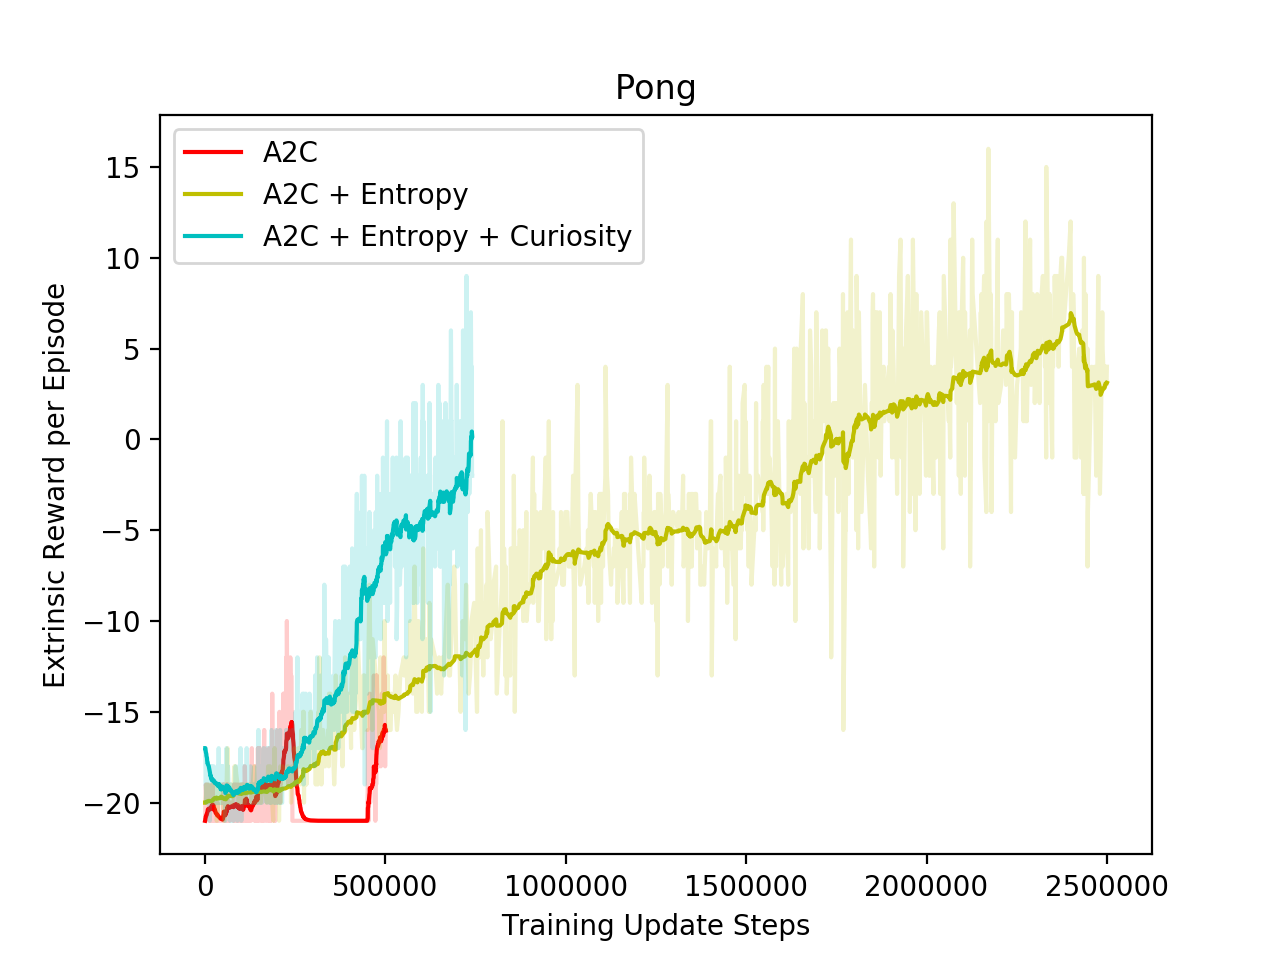
\includegraphics[width=0.6\textwidth]{figures/pong_rewards}
  \caption{We compare the three variants of A2C here, with the curious learner (cyan) vastly outperforming the baseline A2C (red) and the random entropy-based learner (yellow). The extrinsic reward is total cumulative reward over a full episode.}
  \label{fig:pong-reward}
\end{figure}

Relative to the other environments we tested in, \texttt{Pong} provides a much sparser extrinsic reward signal as a positive reward is provided only when the agent is able to score a point, which is a large hurdle during early training. So, in the beginning, much is dependent on the negative reward signal provided only each time the agent allows a point. Most environment steps, in fact, provide a zero reward and so the addition of an intrinsic reward (as with ICM) will become the dominant learning signal, pushing the agent to explore unfamiliar states.

As shown in Fig. \ref{fig:pong-reward}, the curiosity-driven learner trains much faster than the entropy-based learner, which can be explained by the difference in the style of exploration. ICM provides a direct learning signal to the model that encourages the policy to map to actions that are more likely to enter novel, unseen states. In contrast, the entropy term aims to distribute the output probabilities over the next-actions in the policy output space as evenly as possible, preventing the agent from becoming stuck but does so by encouraging the actor to select random actions at times. This difference perhaps explains the higher potential of the curious model, in that it is able to reach higher cumulative rewards that are highly improbable for the entropy-based model.

Note that the cumulative reward in \texttt{Pong} is the the agent's score minus the cpu's score, and the episode ends when either reaches a score of $21$. Thus, the only possible values for cumulative reward are integers between $-21$ and $21$. However, a score of $21$ means that the agent did not allow a single point, and so higher rewards are progressively more and more difficult to reach. This explains the plateauing of model performance at higher rewards, and perhaps also the entropy-based learner's sudden drop near the end of training.

Looking at the baseline A2C model (red in Fig. \ref{fig:pong-reward}), performance is poor due to the fact that the agent has no exploration factor; thus, it tends to get stuck in states where the policy action is to remain in a similar state. This can be seen in the portions of the learning curve where performance collapses and remains stuck for some time.

\subsubsection{Dense Extrinsic Reward}
\begin{figure}
\centering
\begin{subfigure}{.5\textwidth}
  \centering
  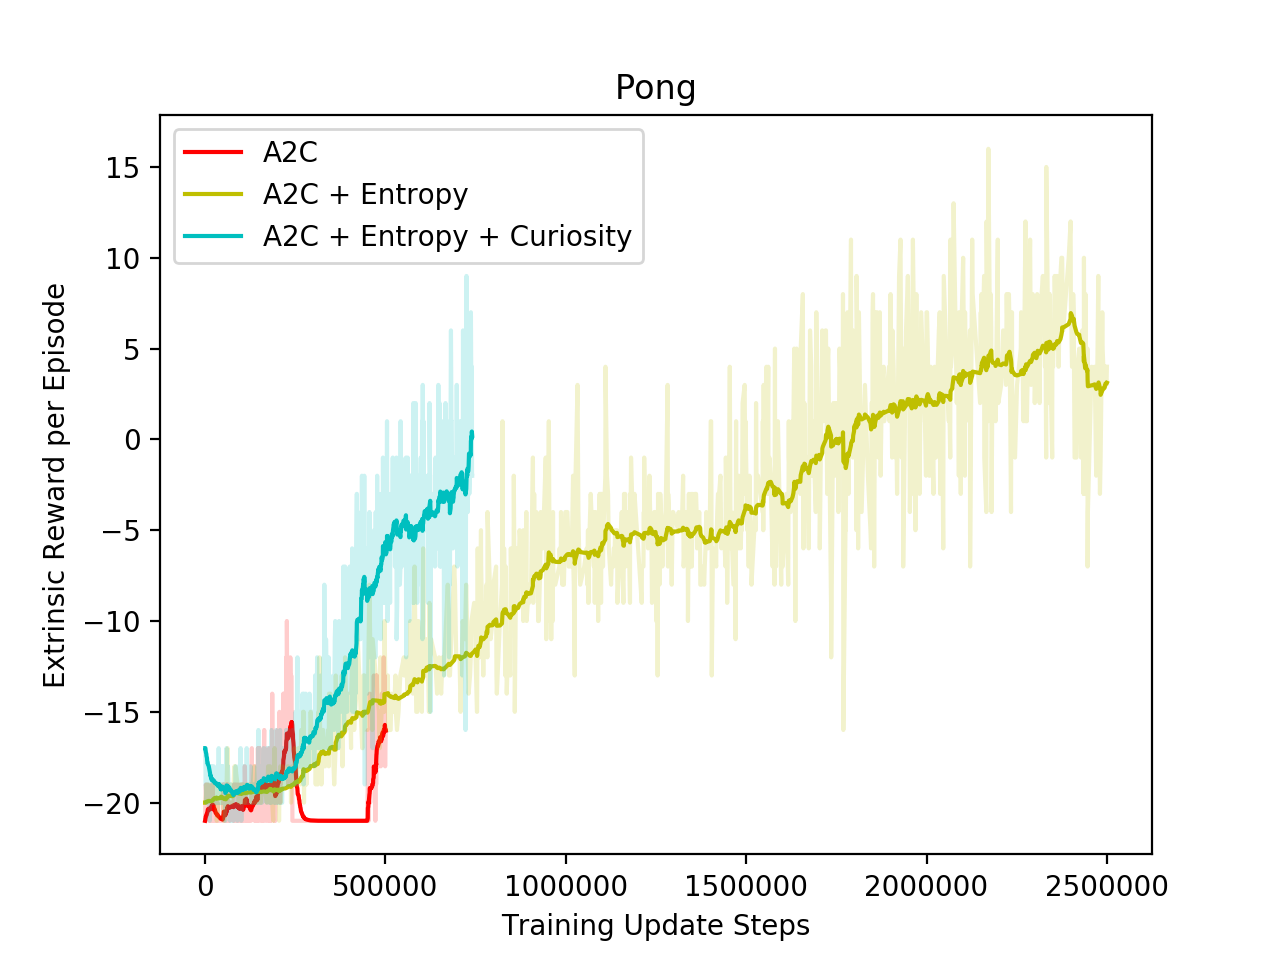
\includegraphics[width=1.\linewidth]{figures/pong_rewards}
\end{subfigure}%
\begin{subfigure}{.5\textwidth}
  \centering
  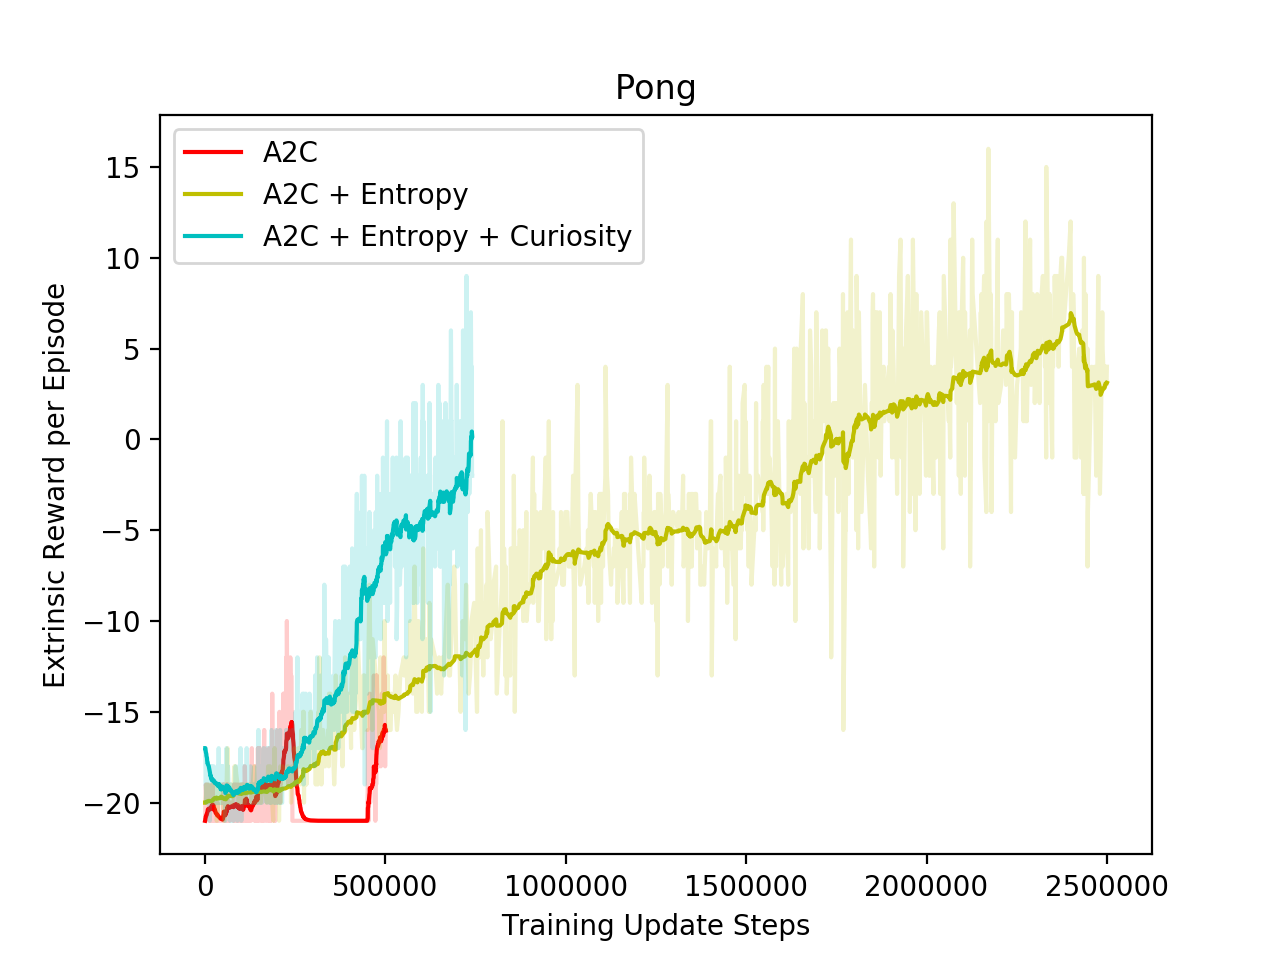
\includegraphics[width=1.\linewidth]{figures/pong_rewards}
\end{subfigure}
\caption{Here we compare the three A2C variants in the \texttt{Breakout} (left) and \texttt{Seaquest} (right) environments. Rewards are again cumulative over an entire episode.}
\label{fig:seaquest-breakout-reward}
\end{figure}

We refer to \texttt{Breakout} and \texttt{Seaquest} as our dense reward environments. Specifically, \texttt{Seaquest} is most dense in that positive rewards are given for each ``kill'', which occurs very frequently due to the sheer number of enemies and the fact that the player's submarine is always firing projectiles at high velocity. In fact, positive rewards are already obtained in the early steps of training (as can be seen in Fig. \ref{fig:seaquest-breakout-reward}). \texttt{Breakout} provides a slightly sparser reward but is still denser than that of \texttt{Pong}; rewards are given for each brick broken which occurs every time the agent is able to return the ball. This means that in early training, when the agent is unable to consistently return the ball, there is no reward signal and so training performance is heavily dependent on an exploration factor.

We note that curiosity related hyper-parameters were not tuned at all for these environments and so the ICM performance remains an area of improvement, particularly in the variance of the intrinsic rewards. This may be the reasoning for the poor performance of the curious learner compared to the entropy-based learner and we hope to address this in future work. It can also be said that the benefits of an intrinsic curiosity-driven reward in environments with dense extrinsic rewards are not as substantial as in sparse reward environments, where the agent often depends on the intrinsic reward as the only learning signal.

Further, the baseline A2C models perform very poorly in these environments, as they again tend to get stuck in certain states (this behaviour can be seen later in the qualitative results). This leads to sudden mode collapse as in the \texttt{Seaquest} environment and an inability to reach further than a score of 10 in \texttt{Breakout} (sharp plateau in reward learning curve). However, relative to the performance in the sparse \texttt{Pong} environment, the baseline A2C model seems to fare better in these dense reward environments thanks to the consistent learning signal.

\subsection{Qualitative Results}
For each trained environment, two agents were considered to investigate the effects of exploration. One artificial agent would be trained without exploration and the other would be trained with exploration. Videos of the agents playing the game in the environment were generated, and through these videos, qualitative observations are made with regards to the effects of exploration, and any interesting behaviours that are seen in the agents that leverage exploration.

\subsubsection{Qualitative Effects of Exploration}

\subsubsubsection{\textbf{Pong}}
\begin{figure}
\centering
\begin{subfigure}{.5\textwidth}
  \centering
  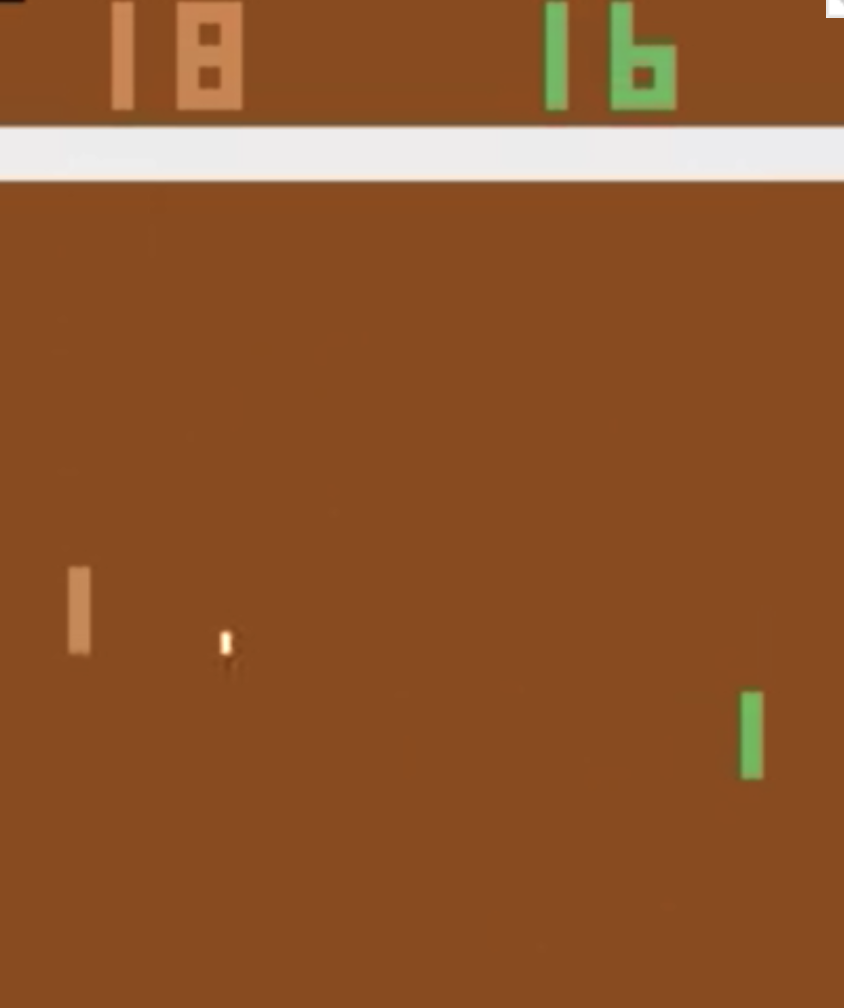
\includegraphics[width=.7\linewidth]{figures/pong}
  \caption{With Exploration}
\end{subfigure}%
\begin{subfigure}{.5\textwidth}
  \centering
  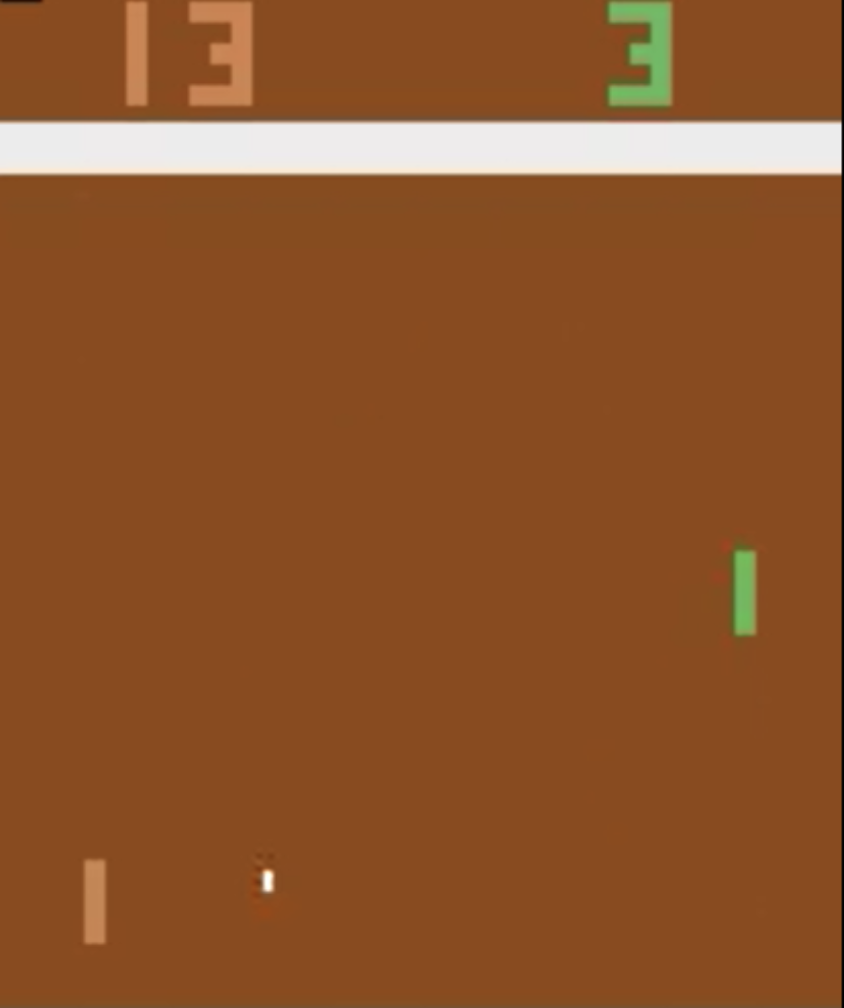
\includegraphics[width=.7\linewidth]{figures/pong_no_exp}
  \caption{Without Exploration}
\end{subfigure}
\caption{Pong environment visualizations}
\label{fig:pong}
\end{figure}
With regards to \texttt{Pong}, the environment with the sparsest rewards from the three that are investigated in this paper, both agents without and with exploration respectively still make use of movement of the paddle to maximize cumulative reward as can be seen in Fig \ref{fig:pong}. However, the agent with exploration noticeably has a much higher rate of movement compared to the agent without exploration, which could lead to more states of the environment being explored. The agent with exploration often makes many movements that are much faster than the agent without exploration, as can be observed in the supplementary videos.

\subsubsubsection{\textbf{Breakout}}
\begin{figure}
\centering
\begin{subfigure}{.5\textwidth}
  \centering
  
\includegraphics[width=.7\linewidth]{figures/breakout}
  \caption{With Exploration}
\end{subfigure}%
\begin{subfigure}{.5\textwidth}
  \centering
  
\includegraphics[width=.7\linewidth]{figures/breakout_no_exp}
  \caption{Without Exploration}
\end{subfigure}
\caption{Breakout environment visualizations}
\label{fig:breakout}
\end{figure}
With regards to \texttt{Breakout}, the environment out of the three investigated in this paper with a higher reward density than \texttt{Pong} but a lower reward density than \texttt{Seaquest}, there is a very noticeable difference in the behaviour of the two agents. The agent without exploration tends to move to the rightmost corner, and simply stay there for most of the game’s duration as can be seen in Fig. \ref{fig:breakout}. The agent with exploration makes movements all across the screen in order to maximize cumulative reward, and intuitively, explores its environment much more than the agent without exploration. This is a very distinct difference in behaviour that can be clearly observed, especially in the supplementary videos provided.

\subsubsubsection{\textbf{Seaquest}}
\begin{figure}
\centering
\begin{subfigure}{.5\textwidth}
  \centering
  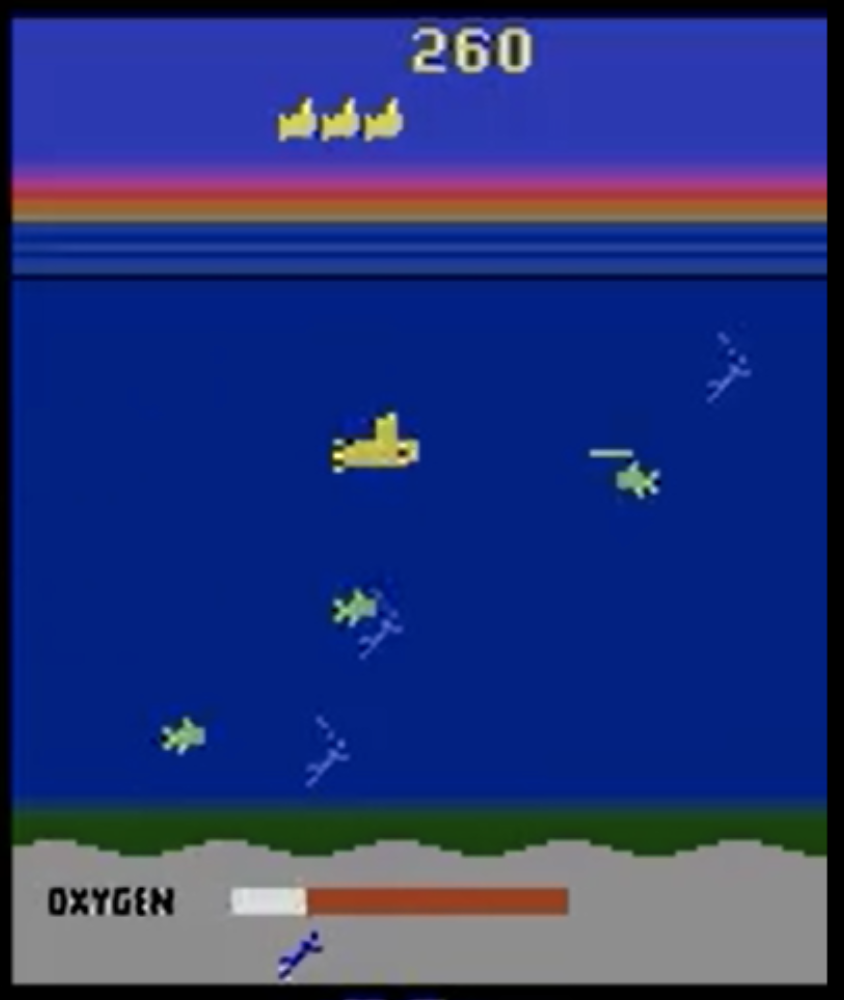
\includegraphics[width=.7\linewidth]{figures/seaquest}
  \caption{With Exploration}
\end{subfigure}%
\begin{subfigure}{.5\textwidth}
  \centering
  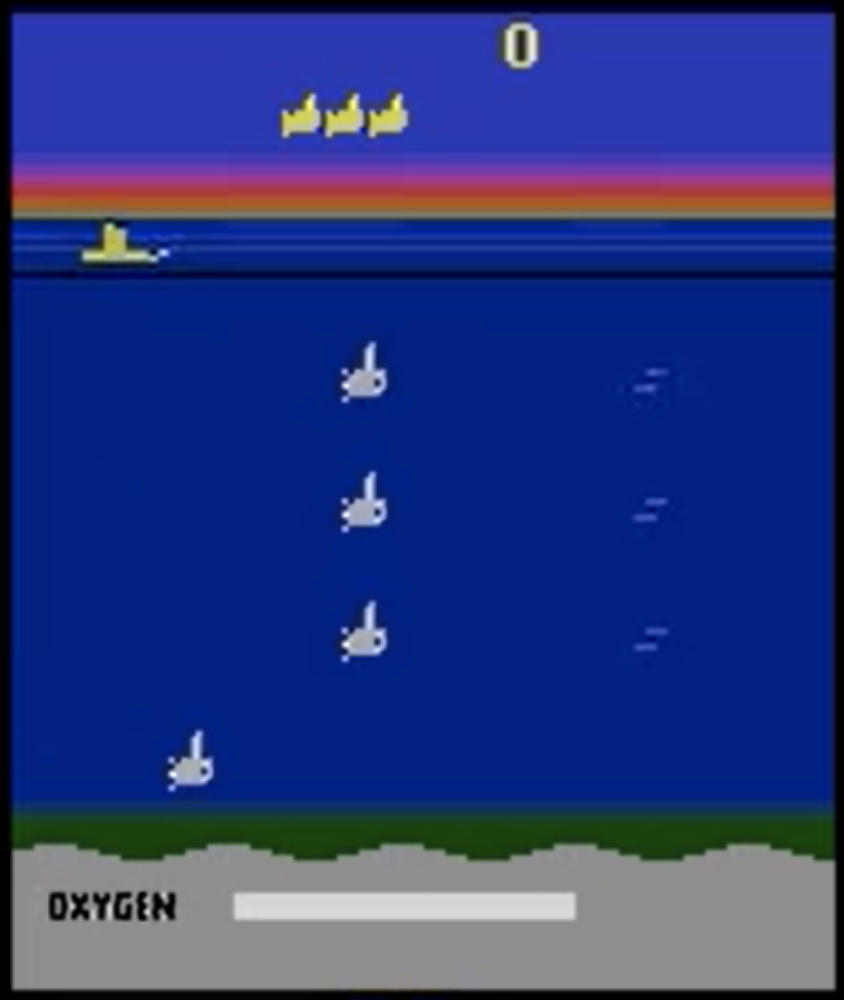
\includegraphics[width=.7\linewidth]{figures/seaquest_no_exp}
  \caption{Without Exploration}
\end{subfigure}
\caption{Seaquest environment visualizations}
\label{fig:seaquest}
\end{figure}
With regards to \texttt{Seaquest}, the environment with the highest reward density, there is also a very noticeable difference in the behaviour of the agents as seen in Fig. \ref{fig:seaquest}. This difference between the two agents is the same as the difference noticed in the agents of \texttt{Breakout}. The agent without exploration in Seaquest does not explore its environment at all, and instead opts to stay above sea level at the top left corner. This behaviour is quite unique because it completely avoids any negative rewards in the environment caused by the fish attacking the agent or due to oxygen loss. On the other hand, the agent with exploration makes movements to fully explore the environment to maximize reward while taking the risk of negative rewards as well.

The differences in behaviour noticed in the agents with and without exploration of both \texttt{Breakout} and \texttt{Seaquest} could perhaps be explained by the lack of maximizing the entropy of the next-action sampling distribution in the agent without exploration. Without this maximization of entropy of the next-action sampling distribution, there is no degree of randomness in the policy network’s state to action mapping. In turn, the lack of randomness may be causing a collapse in the explorative behaviour due to some, perhaps static, actions having a very high probability defined by the policy network logits.

\subsubsection{Interesting Behaviours}

Along with the differences observed in the agents with and without exploration, there are also interesting behaviours observed in the agents with exploration with regards to how they interact with their respective environments. These can be seen in the supplementary videos provided.

In \texttt{Pong}, it is observed that the agent waits for the ball for a bit, and then rapidly moves towards the ball to hit it with the edge of the paddle in order to launch the ball quickly off of the paddle with a high velocity. Perhaps this is a strategy used by the agent to cause a rapid change in velocity that causes the opponent to be unable to catch it in time due to slower reaction speeds.

In \texttt{Breakout}, it is observed that the agent tends to hit the ball from the rightmost corner if it can. This might be a strategy used to break apart the bricks at the top left corner in order to push the ball on top of the bricks, and consequently destroy many more bricks from above in order to accumulate much higher rewards.

In \texttt{Seaquest}, it is observed that the agent takes into consideration the oxygen bar, which is a purely visual indicator. The agent decides the next actions based on their oxygen remaining as well, opting to return to the surface of the water to regain oxygen in order to further extend the opportunity to accumulate more rewards.

\section{Discussion}
Even with the massive computational resources available today, artificial agents face difficulty in balancing explicit exploration of the environment and stable convergence towards a useful, learned policy. In this work, we explored a general formulation of curiosity that aims to motivate the exploration in reinforcement learning agents while remaining invariant to the algorithm and problem in question. This general formulation of curiosity was applied to the A2C RL algorithm in various environments with different extrinsic reward densities to examine the effects of an entropy term (of the policy action probability distribution) and a curiosity module providing an intrinsic reward signal.

As discussed in the results section above, the curiosity-driven (ICM) agents in \texttt{Pong} learn and train much faster than the entropy-based agents, which was explained by the difference in the style of exploration. Moreover, the baseline A2C model with no exploration performed poorly due to the fact that the agent was not exploring at all. With regards to \texttt{Breakout} and \texttt{Seaquest}, particularly dense reward environments, the ICM performance remains an area of improvement through hyper-parameter tuning. The baseline A2C models perform poorly in these environments as discussed previously, but they perform better in these environments relative to sparse reward environments like \texttt{Pong}. Our results show that exploration factors applied to baseline algorithms can improve model performance and decrease training time through intrinsic reward signals. In particular, exploration is crucial across sparse reward environments, which we wanted to verify and which is backed by our results.

The limitations we faced in our work were mostly related to time available to complete this work. With more time, we would have liked to train all of  our agents for longer periods of time until convergence. Moreover, we would prefer to have done more experiments with more time to observe the quantitative effects of hyperparameter tuning for specific environments such as \texttt{Breakout} and \texttt{Seaquest} and agents with intrinsic curiosity (ICM) since we were unable to do so in the time we had. 

In the future, we would like to diversify the environments investigated in this paper. \texttt{Pong}, \texttt{Breakout}, and \texttt{Seaquest} are all Atari games where the states and frames of the game do not change drastically from one state to another. This could perhaps be a factor affecting the ICM due to the fact that novelty in states for curiosity is defined by the change in its features. Through more experiments in a diversified set of environments including environments with more distinct states, additional insights about the effect of exploration and curiosity might be revealed.

\bibliography{main}
\bibliographystyle{ieeetr}

\end{document}
